\documentclass[11pt]{homework}

\usepackage[UTF8]{ctex}
\usepackage{graphicx}
\usepackage{float} 
\usepackage{subfigure}
\usepackage{color}
\usepackage{listings}
\lstset{
  showspaces=false,
  showtabs=false,
  breaklines=true,
  showstringspaces=false,
  breakatwhitespace=true,
  commentstyle=\color{green},
  keywordstyle=\color{blue},
  stringstyle=\color{red},
  basicstyle=\ttfamily,
  moredelim=[il][\textcolor{pgrey}]{$$},
  moredelim=[is][\textcolor{pgrey}]{\%\%}{\%\%}
}

\newcommand{\hwname}{封钰震}
\newcommand{\hwemail}{1951362}
\newcommand{\hwtype}{作业}
\newcommand{\hwnum}{4-Java GUI}
\newcommand{\hwclass}{Java语言程序设计}
\newcommand{\hwlecture}{}
\newcommand{\hwsection}{}

\usepackage{lipsum}

\begin{document}
\maketitle

\section*{编程环境}

  \subsection*{硬件环境}
  \begin{itemize}
    \item 型号名称:MacBook Pro
    \item 处理器名称:Dual-Core Intel Core i5
    \item 内存:8 GB
  \end{itemize}

  \subsection*{软件环境}
  \begin{itemize}
    \item 操作系统:macOS 10.15.7
  \end{itemize}

  \subsection*{运行环境}
  \begin{itemize}
    \item JDK 14.0.2
  \end{itemize}

\section*{设计思想}

  \subsection*{窗口布局}
  首先从\verb|JFrame|继承一个名为\verb|TextComponentFrame|类作为我们的窗口容器。在这个\verb|TextComponentFrame|中包括2个\verb|JPanel|面板容器(分别名为\verb|filePanel|和\verb|stylePanel|)和1个\verb|JScrollPane|滚动面板容器(名为\verb|scrollPane|)。

  \verb|filePanel|面板容器分别容纳与加载和保存文件有关的组件(用于第一问),包括输入文件名的文本域\verb|fileNameField|、“加载文件”按钮\verb|loadFileButton|、“保存文件”按钮\verb|saveFileButton|。

  \verb|stylePanel|面板容器分别容纳与更改、加载和保存样式有关的组件(用于第二、三问),包括用于选择样式的组合框、滑动条,输入样式文件名的文本域\verb|styleFileNameField|,“更改样式”按钮\verb|changeStyleButton|,“加载样式”按钮\verb|loadStyleButton|,“保存样式”按钮\verb|saveStyleButton|。

  \verb|scrollPane|滚动面板容器包含了一个文本区\verb|contentArea|。

  \subsection*{事件触发}
  对于窗口中的每一个按钮,调用\verb|addActionListener|方法,设置一个监听器。每一个监听器都是一个内部类,实现了\verb|ActionListener|接口。当按钮被按下时,监听器的\verb|actionPerformed|方法就会被调用。

  对于“加载文件”按钮\verb|loadFileButton|,被点击后,若文件存在,则会设置文本区\verb|contentArea|的内容为文件内容;若文件不存在,则会弹出弹窗询问用户是否需要新建文件,若用户点击“是”,则新建文件。

  对于“保存文件”按钮\verb|saveFileButton|,被点击后,则保存\verb|contentArea|的内容至\verb|fileNameField|路径文件下。

  对于“更改样式”按钮\verb|changeStyleButton|,被点击后,则设置窗口样式为用户选择的样式。

  对于“加载样式”按钮\verb|loadStyleButton|,被点击后,若文件存在,则会加载文件中的样式属性,并设置为窗口样式;若文件不存在,则会弹出弹窗提示用户。

  对于“保存样式”按钮\verb|saveStyleButton|,被点击后,则保存当前用户设置的样式至\verb|styleFileNameField|路径文件下。

  \subsection*{样式文件}
  样式文件的示例如下:
  \begin{lstlisting}
    #Style Settings
    #Sun Nov 14 23:33:00 CST 2021
    loc=\u4E0A\u4E0B\u5E03\u5C40
    size=36
    fontStyle=0
    font=Segoe UI
  \end{lstlisting}

  其中,第1-2行为注释,第3行为组件布局(Unicode编码),第4行为字体大小,第5行为字型,第6行为字体。

\section*{执行过程}

  完整的窗口如图\ref{窗口}所示。

  \begin{figure}
    \centering
    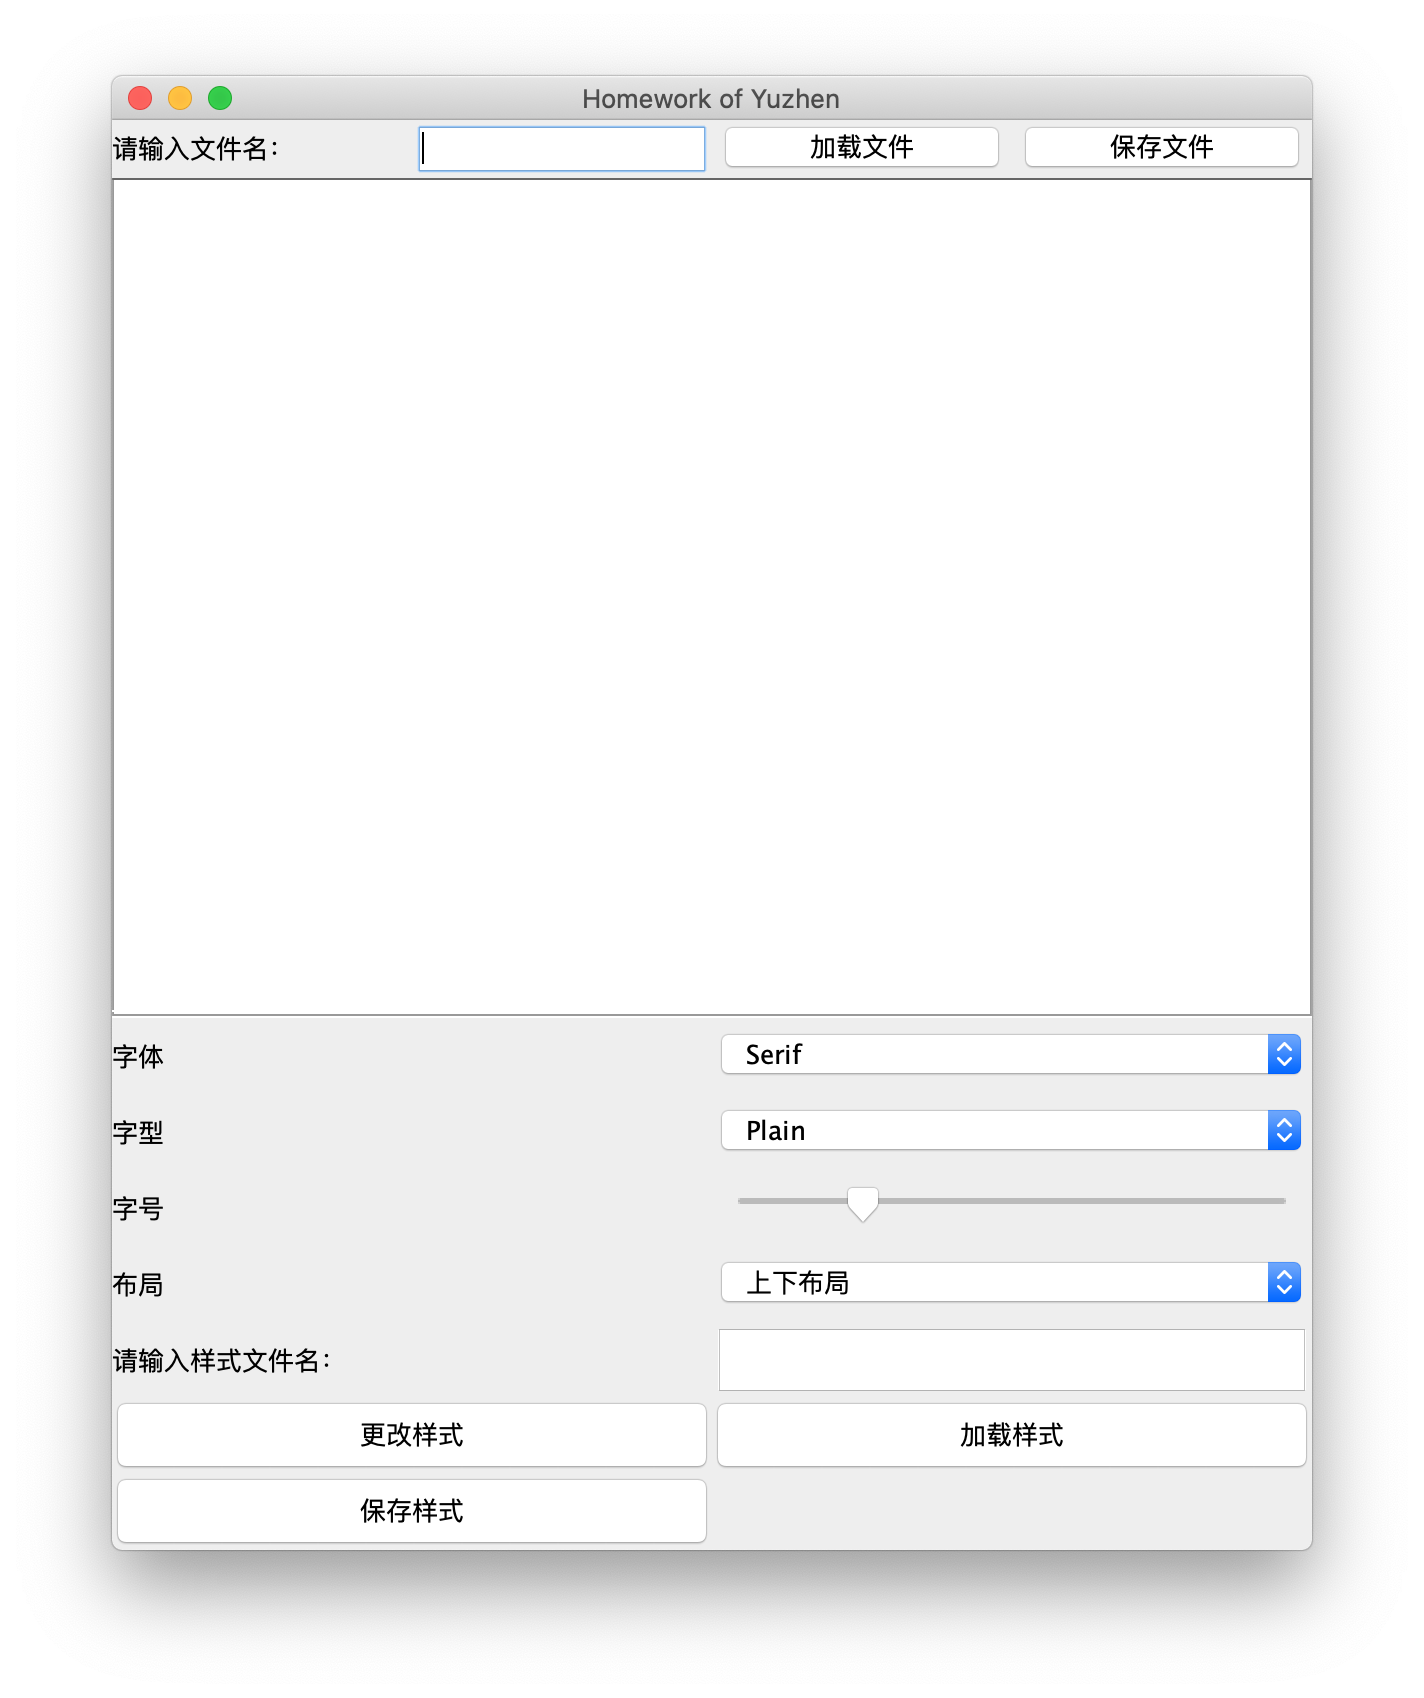
\includegraphics[width=0.5\textwidth]{窗口}
    \caption{窗口}
    \label{窗口}
  \end{figure}

  \subsection*{第一问}

  首先,在文本域中输入一个不存在的文件路径,点击“加载文件”。此时,会弹窗提示“文件不存在,是否要新建文件?”,如图\ref{文件不存在}所示。点击“是”后,创建文件。在文件中输入内容,点击“保存文件”,则弹窗提示“文件保存成功!”,如图\ref{文件保存成功}所示。输入一个存在的文件路径,重新“加载文件”,弹窗提示“文件加载成功!”,如图\ref{文件加载成功}所示。然后看到文本区中加载了文件中的内容,如图\ref{文件存在}所示。

  \begin{figure}
    \centering
    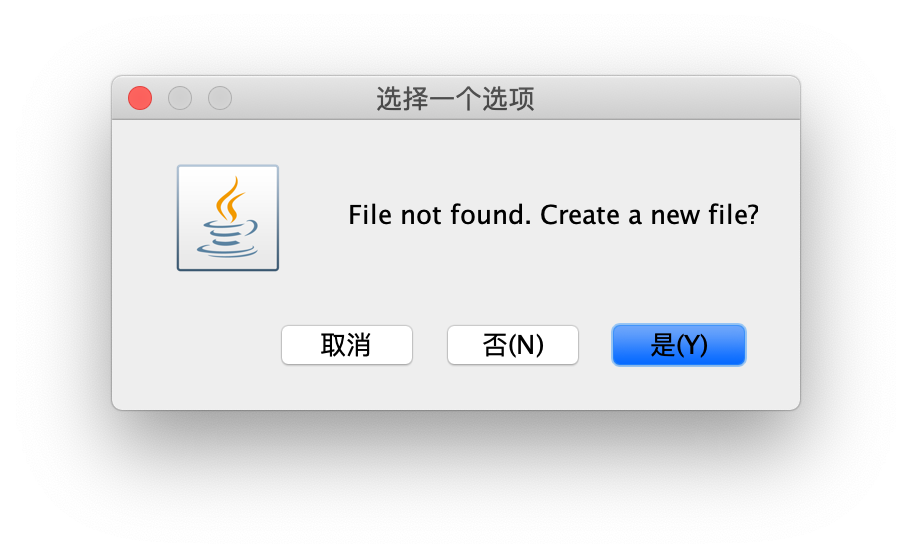
\includegraphics[width=0.5\textwidth]{文件不存在}
    \caption{文件不存在}
    \label{文件不存在}
  \end{figure}

  \begin{figure}
    \centering
    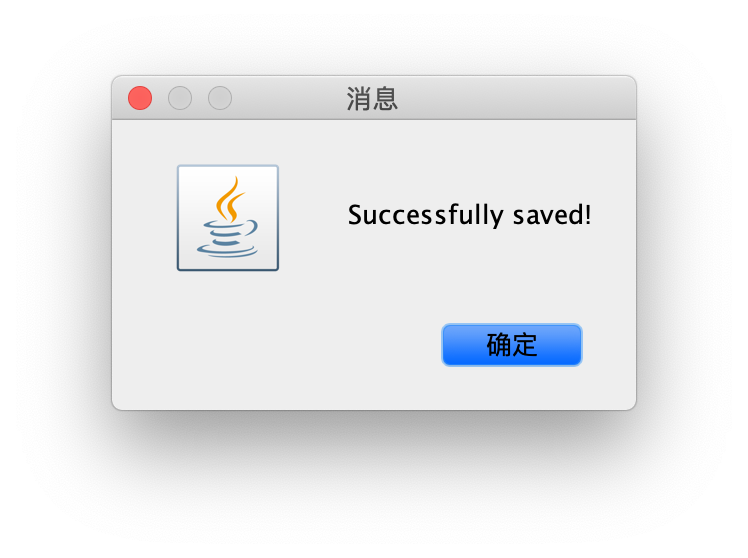
\includegraphics[width=0.5\textwidth]{文件保存成功}
    \caption{文件保存成功}
    \label{文件保存成功}
  \end{figure}

  \begin{figure}
    \centering
    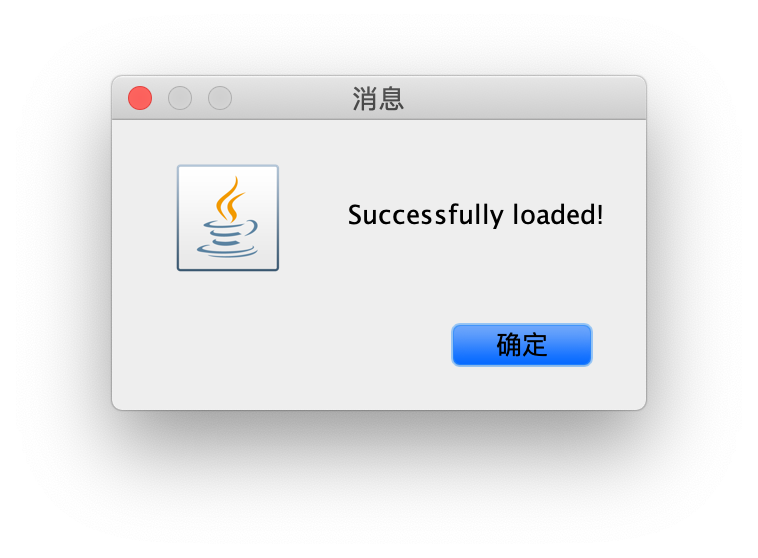
\includegraphics[width=0.5\textwidth]{文件加载成功}
    \caption{文件加载成功}
    \label{文件加载成功}
  \end{figure}

  \begin{figure}
    \centering
    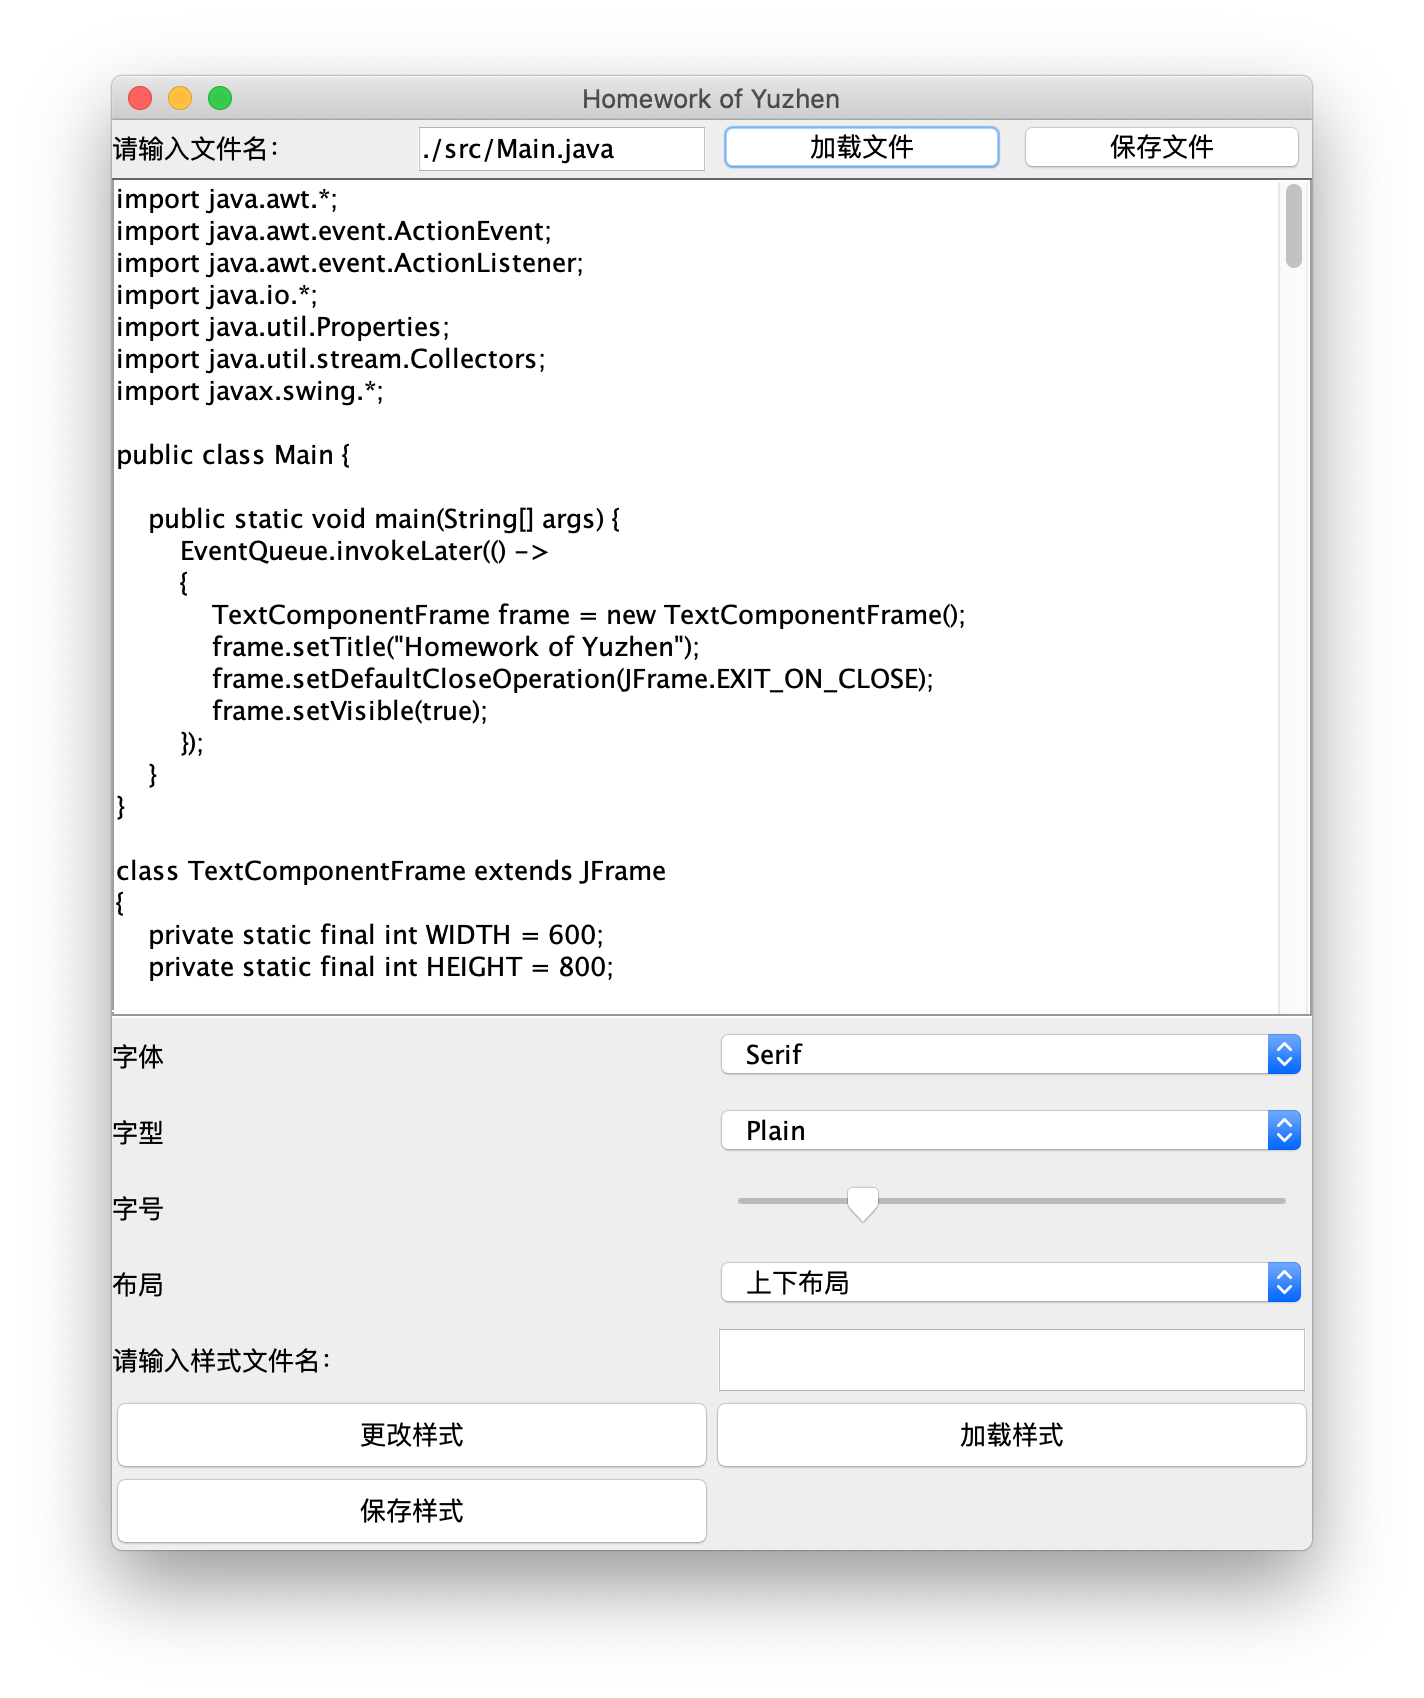
\includegraphics[width=0.5\textwidth]{文件存在}
    \caption{文件存在}
    \label{文件存在}
  \end{figure}
  
  \subsection*{第二问}

  可以通过\verb|stylePanel|面板容器中的组件调整样式,如图\ref{风格切换1}和图\ref{风格切换2}所示。

  \begin{figure}
    \centering
    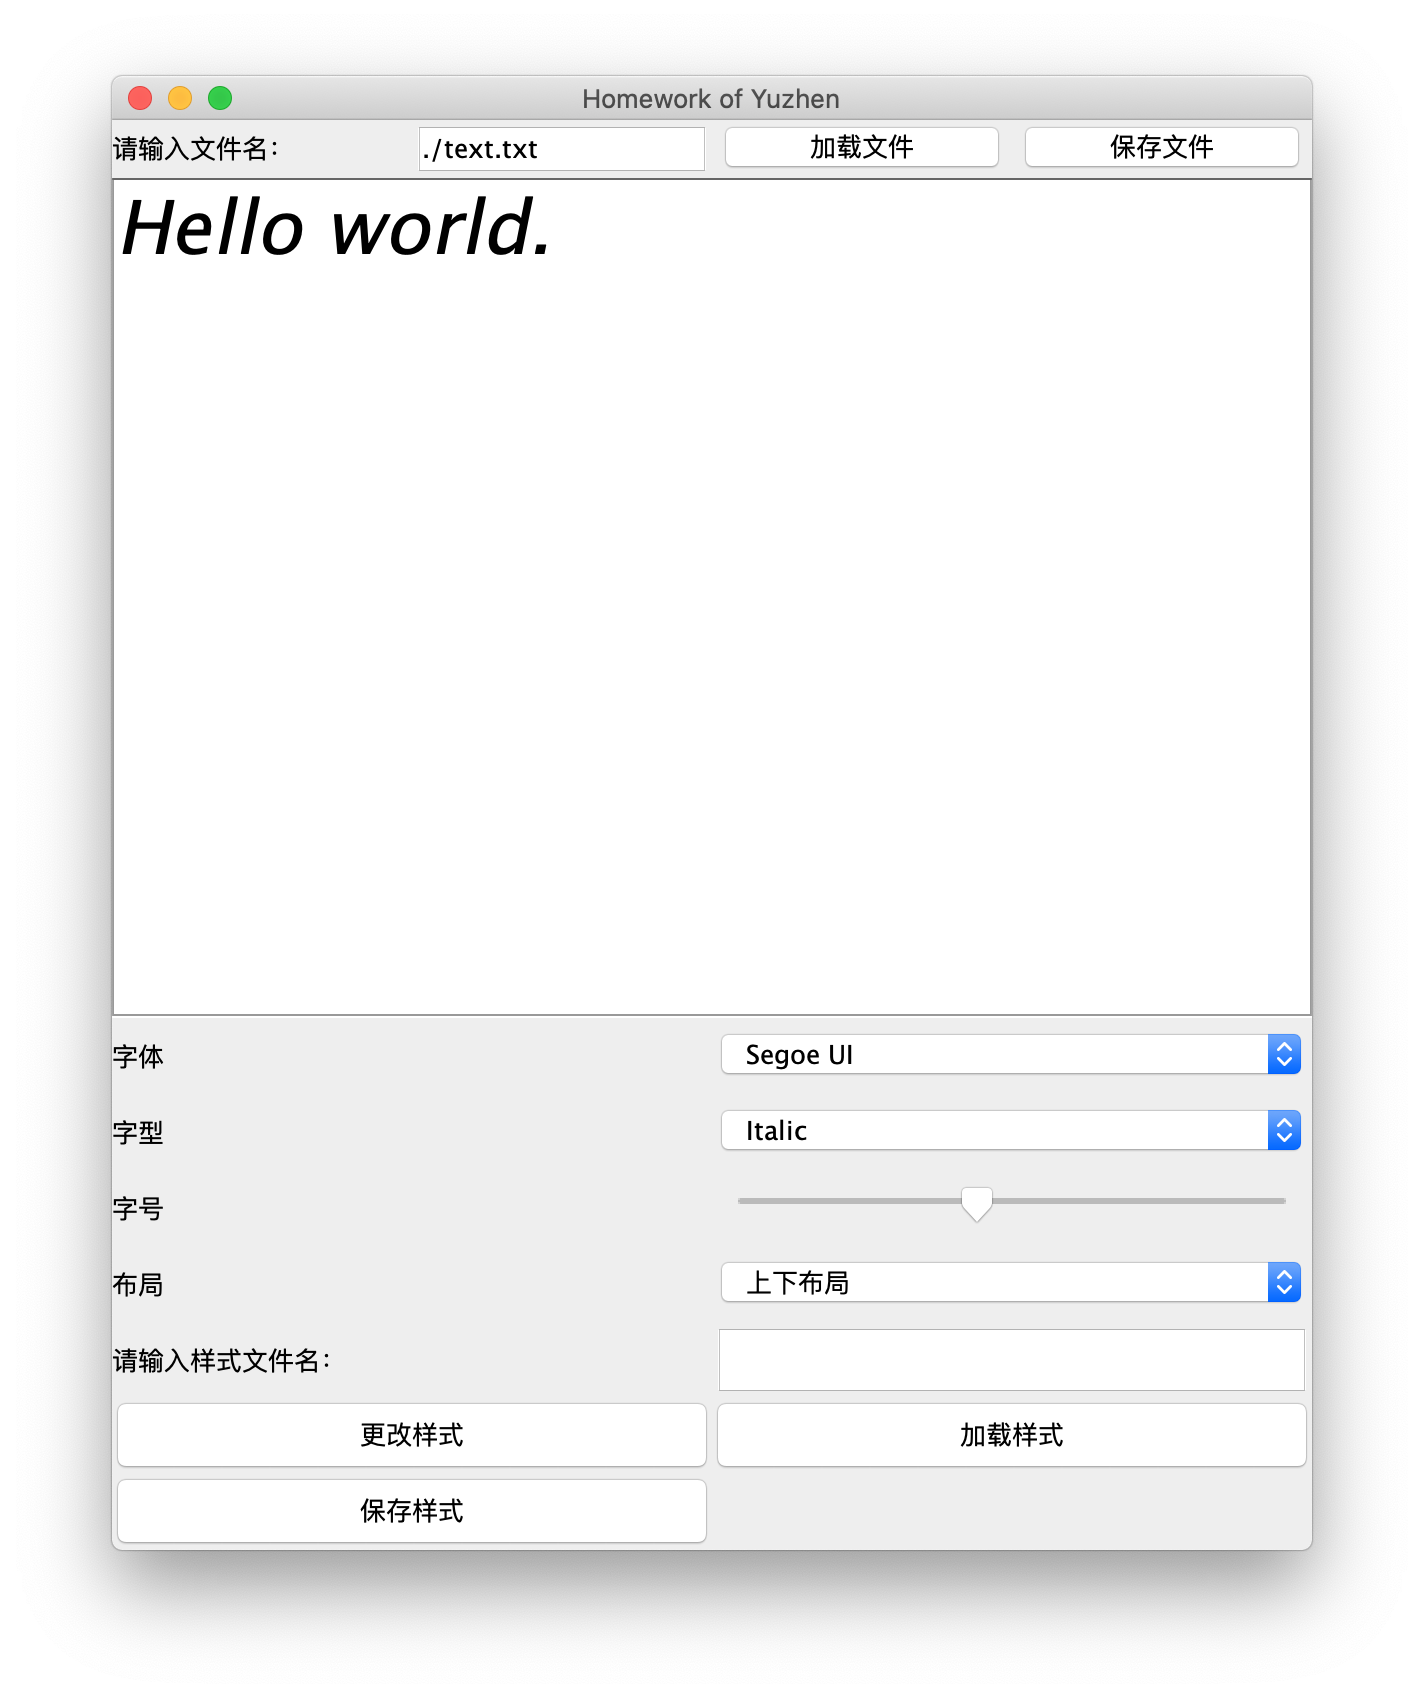
\includegraphics[width=0.5\textwidth]{风格切换1}
    \caption{风格切换1}
    \label{风格切换1}
  \end{figure}

  \begin{figure}
    \centering
    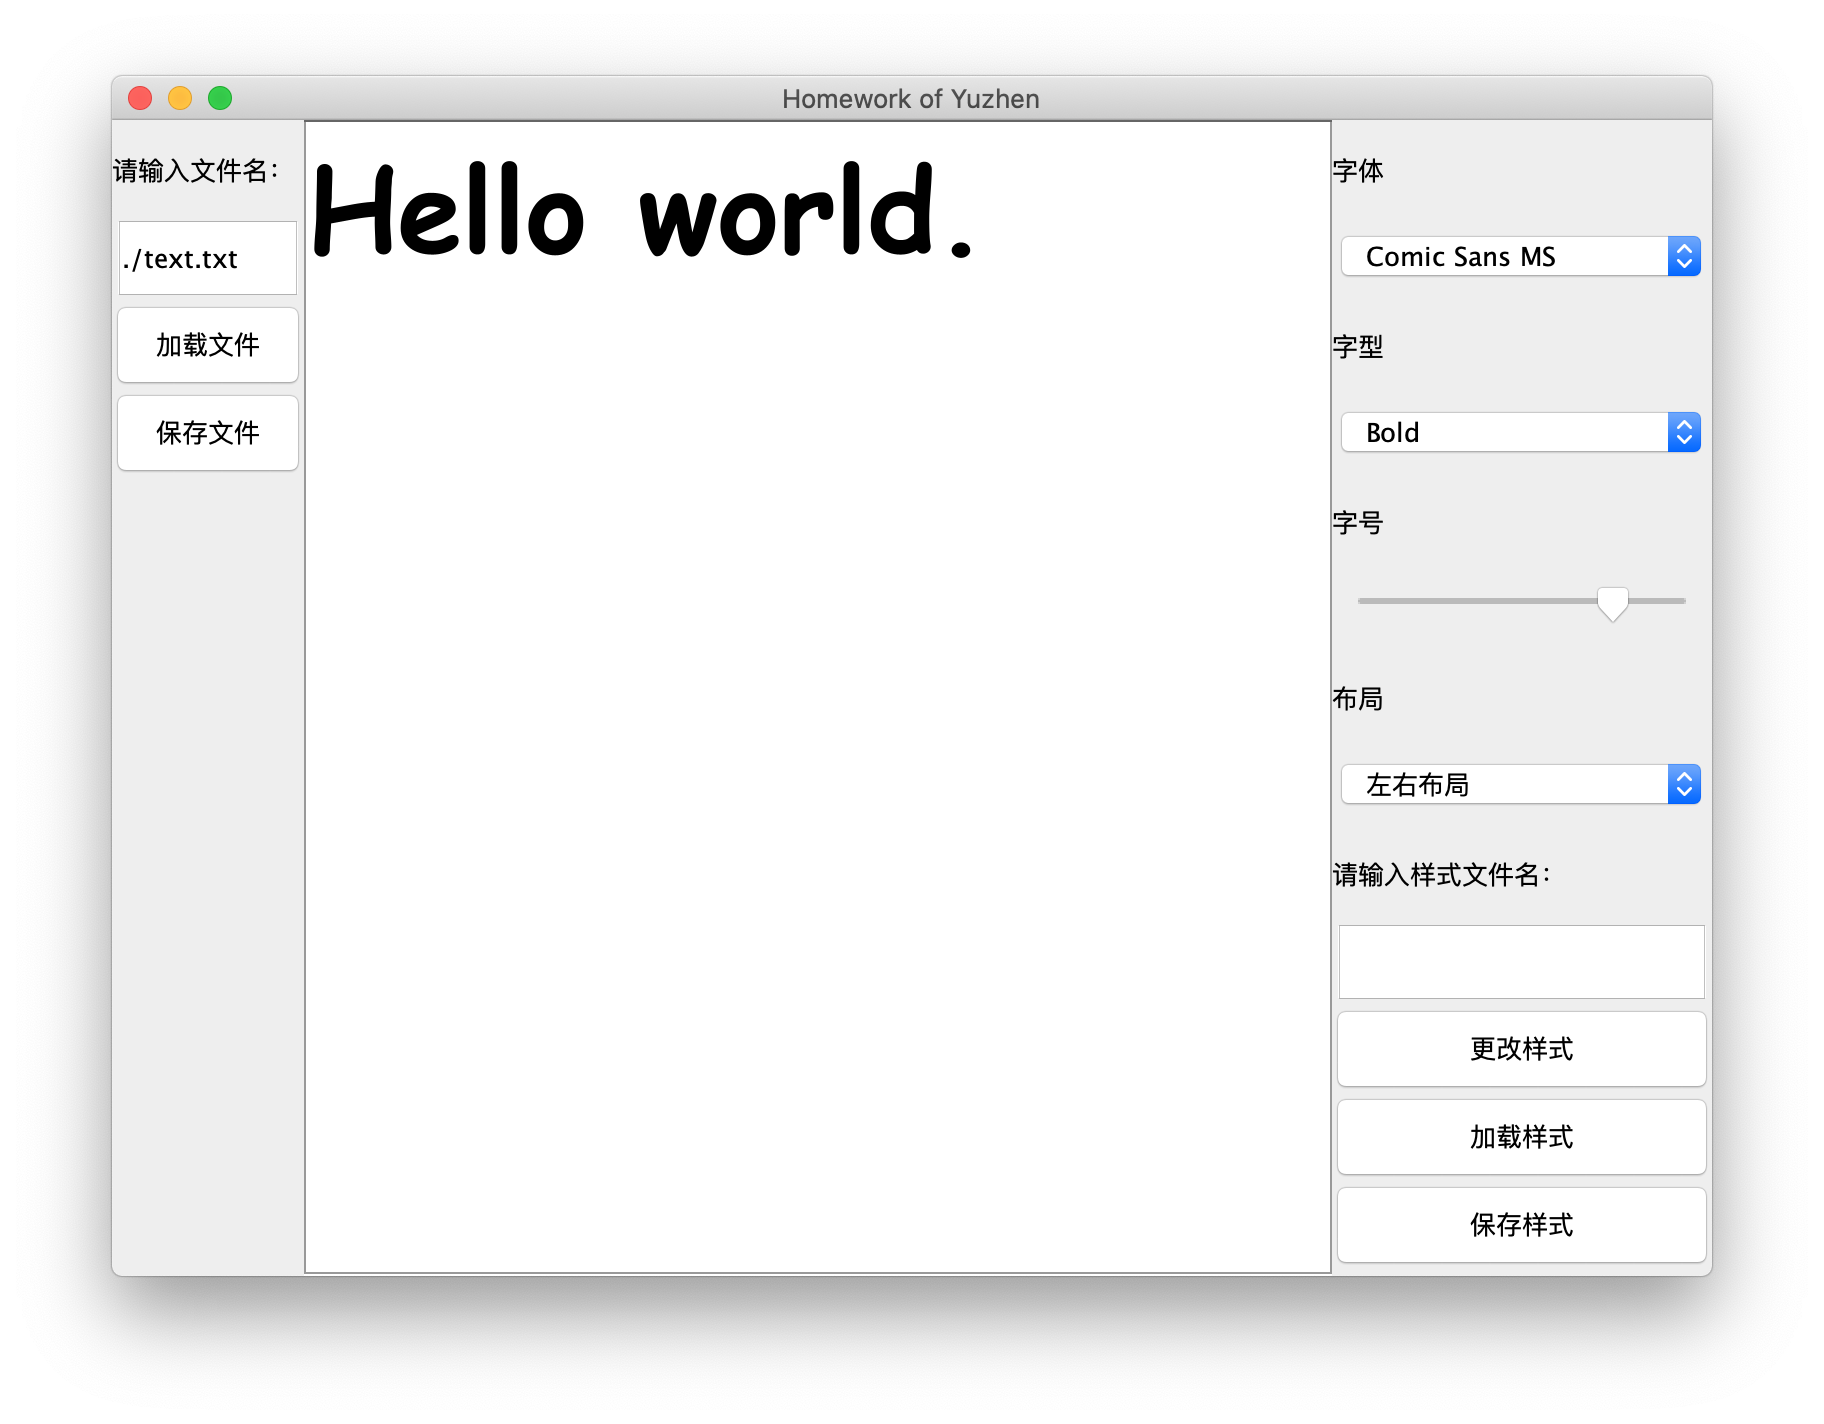
\includegraphics[width=0.5\textwidth]{风格切换2}
    \caption{风格切换2}
    \label{风格切换2}
  \end{figure}

  \subsection*{第三问}

  若要保存当前样式,则输入配置文件保存路径,点击“保存样式”,则将样式保存到目标路径中。对于图\ref{风格切换2}中的样式,配置文件即为:
  \begin{lstlisting}
    #Style Settings
    #Mon Nov 15 10:59:12 CST 2021
    loc=\u5DE6\u53F3\u5E03\u5C40
    size=58
    fontStyle=1
    font=Comic Sans MS
  \end{lstlisting}

  若要加载配置文件中的样式,则输入其路径,点击“加载样式”即可。

\section*{窗口类源代码}

\lstset{language=Java}
\begin{lstlisting}
  class TextComponentFrame extends JFrame
  {
      private static final int WIDTH = 600;
      private static final int HEIGHT = 800;
  
      private JPanel filePanel;
      private JTextField fileNameField;
      private JButton loadFileButton;
      private JButton saveFileButton;
  
      private JScrollPane scrollPane;
      private JTextArea contentArea;
  
      private JPanel stylePanel;
      private JComboBox<String> fontOpt;
      private JComboBox<String> fontStyleOpt;
      private JSlider sizeOpt;
      private JComboBox<String> locOpt;
      private JTextField styleFileNameField;
      private JButton changeStyleButton;
      private JButton loadStyleButton;
      private JButton saveStyleButton;
  
      private void setStyle(String font, int fontStyle, int size, String loc)
      {
          contentArea.setFont(new Font(font, fontStyle, size));
          switch (loc) {
              case "左右布局": {
                  getLayout().removeLayoutComponent(filePanel);
                  getLayout().removeLayoutComponent(stylePanel);
                  setSize(HEIGHT, WIDTH);
                  filePanel.setLayout(new GridLayout(13, 1));
                  stylePanel.setLayout(new GridLayout(13, 1));
                  add(filePanel, BorderLayout.WEST);
                  add(stylePanel, BorderLayout.EAST);
                  add(scrollPane, BorderLayout.CENTER);
                  break;
              }
              case "上下布局": {
                  getLayout().removeLayoutComponent(filePanel);
                  getLayout().removeLayoutComponent(stylePanel);
                  setSize(WIDTH, HEIGHT);
                  filePanel.setLayout(new GridLayout(1, 4));
                  stylePanel.setLayout(new GridLayout(7, 2));
                  add(filePanel, BorderLayout.NORTH);
                  add(stylePanel, BorderLayout.SOUTH);
                  add(scrollPane, BorderLayout.CENTER);
                  break;
              }
          }
      }
  
      public TextComponentFrame()
      {
          contentArea = new JTextArea();
          contentArea.setLineWrap(true);
          scrollPane = new JScrollPane(contentArea);
  
          filePanel = new JPanel();
          filePanel.setLayout(new GridLayout(1, 4));
          fileNameField = new JTextField();
          loadFileButton = new JButton("加载文件");
          saveFileButton = new JButton("保存文件");
          filePanel.add(new JLabel("请输入文件名:"));
          filePanel.add(fileNameField);
          filePanel.add(loadFileButton);
          filePanel.add(saveFileButton);
  
          stylePanel = new JPanel();
          stylePanel.setLayout(new GridLayout(7, 2));
          fontOpt = new JComboBox<>(new String[]{"Serif", "Agency FB", "Arial", "Calibri", "Cambrian",
                  "Century Gothic", "Comic Sans MS", "Courier New", "Forte", "Garamond",
                  "Monospaced", "Segoe UI", "Times New Roman", "Trebuchet MS"});
          fontStyleOpt = new JComboBox<>(new String[]{"Plain", "Bold", "Italic"});
          sizeOpt = new JSlider(10, 72, 24);
          sizeOpt.setPaintLabels(true);
          sizeOpt.setPaintTicks(true);
          locOpt = new JComboBox<>(new String[]{"上下布局", "左右布局"});
          styleFileNameField = new JTextField();
          changeStyleButton = new JButton("更改样式");
          loadStyleButton = new JButton("加载样式");
          saveStyleButton = new JButton("保存样式");
          stylePanel.add(new JLabel("字体"));
          stylePanel.add(fontOpt);
          stylePanel.add(new JLabel("字型"));
          stylePanel.add(fontStyleOpt);
          stylePanel.add(new JLabel("字号"));
          stylePanel.add(sizeOpt);
          stylePanel.add(new JLabel("布局"));
          stylePanel.add(locOpt);
          stylePanel.add(new JLabel("请输入样式文件名:"));
          stylePanel.add(styleFileNameField);
          stylePanel.add(changeStyleButton);
          stylePanel.add(loadStyleButton);
          stylePanel.add(saveStyleButton);
  
          add(filePanel, BorderLayout.NORTH);
          add(stylePanel, BorderLayout.SOUTH);
          add(scrollPane, BorderLayout.CENTER);
          pack();
  
          loadFileButton.addActionListener(new LoadFileAction());
          saveFileButton.addActionListener(new SaveFileAction());
          changeStyleButton.addActionListener(new ChangeStyleAction());
          loadStyleButton.addActionListener(new LoadStyleAction());
          saveStyleButton.addActionListener(new SaveStyleAction());
  
          setSize(WIDTH, HEIGHT);
          setLocationByPlatform(true);
      }
  
      private class LoadFileAction implements ActionListener
      {
          @Override
          public void actionPerformed(ActionEvent e)
          {
              String fileName = fileNameField.getText();
              String content;
              try {
                  BufferedReader reader = new BufferedReader(new FileReader(fileName));
                  content = reader.lines().collect
                      (Collectors.joining(System.lineSeparator()));
                  reader.close();
                  JOptionPane.showMessageDialog(contentArea, "Successfully loaded!");
              } catch (FileNotFoundException ex)
              {
                  int option = JOptionPane.showConfirmDialog(contentArea, "File not found. Create a new file?");
                  if (option == JOptionPane.YES_OPTION)
                  {
                      try {
                          (new File(fileName)).createNewFile();
                      } catch (IOException ex1) {
                          JOptionPane.showMessageDialog(contentArea, ex1.getMessage());
                      }
                  }
                  content = "";
              } catch (Exception ex)
              {
                  content = "";
                  JOptionPane.showMessageDialog(contentArea, ex.getMessage());
              }
              contentArea.setText(content);
          }
      }
  
      private class SaveFileAction implements ActionListener
      {
          @Override
          public void actionPerformed(ActionEvent e) {
              String fileName = fileNameField.getText();
              BufferedWriter writer;
              try {
                  writer = new BufferedWriter(new FileWriter(fileName));
                  writer.write(contentArea.getText());
                  writer.close();
                  JOptionPane.showMessageDialog(contentArea, "Successfully saved!");
              } catch (IOException ex) {
                  JOptionPane.showMessageDialog(contentArea, ex.getMessage());
              }
          }
      }
  
      private class ChangeStyleAction implements ActionListener
      {
          @Override
          public void actionPerformed(ActionEvent e) {
              String font = (String) fontOpt.getSelectedItem();
              int fontStyle = fontStyleOpt.getSelectedIndex();
              int size = sizeOpt.getValue();
              String loc = (String) locOpt.getSelectedItem();
              setStyle(font, fontStyle, size, loc);
          }
      }
  
      private class LoadStyleAction implements ActionListener
      {
          @Override
          public void actionPerformed(ActionEvent e)
          {
              String fileName = styleFileNameField.getText();
              Properties properties = new Properties();
              try {
                  FileInputStream reader = new FileInputStream(fileName);
                  properties.load(reader);
                  reader.close();
                  JOptionPane.showMessageDialog(contentArea, "Successfully loaded!");
                  String font = properties.getProperty("font", "Serif");
                  int fontStyle = Integer.parseInt(properties.getProperty("fontStyle", "0"));
                  int size = Integer.parseInt(properties.getProperty("size", "24"));
                  String loc = properties.getProperty("loc", "上下布局");
                  setStyle(font, fontStyle, size, loc);
                  fontOpt.setSelectedItem(font);
                  fontStyleOpt.setSelectedItem(fontStyle);
                  sizeOpt.setValue(size);
                  locOpt.setSelectedItem(loc);
              } catch (Exception ex)
              {
                  JOptionPane.showMessageDialog(contentArea, ex.getMessage());
              }
          }
      }
  
      private class SaveStyleAction implements ActionListener
      {
          @Override
          public void actionPerformed(ActionEvent e) {
              String fileName = styleFileNameField.getText();
              Properties properties = new Properties();
              properties.setProperty("font", (String) fontOpt.getSelectedItem());
              properties.setProperty("fontStyle", String.valueOf(fontStyleOpt.getSelectedIndex()));
              properties.setProperty("size", String.valueOf(sizeOpt.getValue()));
              properties.setProperty("loc", (String) locOpt.getSelectedItem());
              try {
                  FileOutputStream writer = new FileOutputStream(fileName);
                  properties.store(writer, "Style Settings");
                  writer.close();
                  JOptionPane.showMessageDialog(contentArea, "Successfully saved!");
              } catch (IOException ex) {
                  JOptionPane.showMessageDialog(contentArea, ex.getMessage());
              }
          }
      }
  }
\end{lstlisting}

\end{document}